\documentclass{article}
\usepackage[UTF8]{ctex} % 用于中文排版
\usepackage{geometry}
\usepackage{indentfirst}
\usepackage{enumitem}

\usepackage{titling}    % 用于自定义标题页
\usepackage{graphicx}
\usepackage{float}

\usepackage{xcolor}
\usepackage{listings}

\usepackage{setspace}
\usepackage{siunitx}    % 单位

% 页面几何设置
\geometry{a4paper, left=25mm, right=25mm, top=25mm, bottom=25mm}
% 取消首行缩进
\setlength{\parindent}{0pt}
% 行间距设置
\setstretch{1.5}
% 自定义字体大小
\newcommand{\fourhao}{\fontsize{14pt}{\baselineskip}\selectfont} % 四号字体
\newcommand{\xiaosihao}{\fontsize{12pt}{\baselineskip}\selectfont} % 小四号字体
\newcommand{\song}{\CJKfamily{song}}
% 设置代码块格式
\lstset{
    basicstyle = \footnotesize\ttfamily,                 % 设置行距,字体
    numbers = left,                                      % 在左侧显示行号
    numberstyle = \tiny \color{gray},                    % 设定行号格式
    keywordstyle = \bfseries \color[RGB]{40,40,255},     % 设定关键字颜色
    numberstyle = \footnotesize \color{darkgray},           
    commentstyle = \color[RGB]{0,96,96},                 % 设置代码注释的格式
    stringstyle = \color[RGB]{128,0,0},                  % 设置字符串格式
    frame = single,                                      % 不显示背景边框
    backgroundcolor = \color[RGB]{245,245,244},          % 设定背景颜色
    language=Verilog                                     % 设置语言
}
\raggedbottom   % 段落间留白, 避免排版时自动拉伸导致的行间距变化。
\begin{document}

% 封面页面
\begin{titlepage}
    \centering
    \vspace*{2cm}

    \Huge
    \textbf{课程名称:EDA 技术综合设计}

    \vspace{2cm}

    \LARGE
    设计报告名称:设计一\ 流水灯

    \vspace{4cm}

    \centering
    \Large
    \begin{tabular}{rl}
        班级: & 通信214    \\
        姓名: & \ 王峤宇    \\
        学号: & \ 214022
    \end{tabular}

    \vfill

    \vspace{1cm}
\end{titlepage}

\newpage
% 第一部分
\section*{\fourhao 一、设计内容及原理}
\xiaosihao
\setstretch{1.5}
% 设计项目内容及设计原理,如真值表、状态表及状态转换图、文字说明等。
设计流水灯, 流水灯的设计是时序逻辑电路, 需要对输入的100MHz时钟进行分频, 
通过计数器进行分频后驱动LED灯的控制寄存器移位, 实现流水灯的效果。
\begin{figure}[htbp]
    \centering
    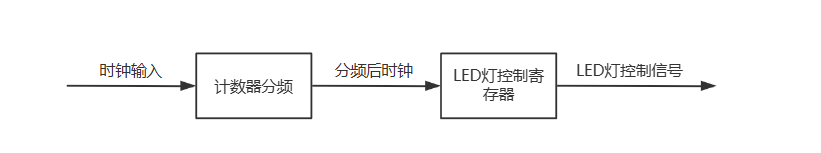
\includegraphics[width=0.7\textwidth]{image/2024-06-28-12-46-01.png}
    \caption{流水灯模块框图}
    \label{image_principle_1}
\end{figure}
流水灯实现模块框图如图\ref{image_principle_1}所示。
\section*{\fourhao 二、设计过程}
\xiaosihao
\setstretch{1.5}
% 从工程建立开始,一直到硬件调试。
% 按照基础任务、提高任务和拓展任务分别给出相应的源文件、仿真文件、约束文件
流水灯源文件添加注释后如下所示:
\begin{lstlisting}[language=Verilog, caption={流水灯源文件}]
module flow_led (
    input clk,          /* 输入时钟 */
    input rst,          /* 复位信号 */
    output [15:0] led   /* 16个led的控制信号 */
    );
    reg [23:0] cnt_reg;     /* 计数器 */
    reg [15:0] light_reg;   /* led控制 */
    always @ (posedge clk) begin
        if(!rst)                    /* 同步复位 */
            cnt_reg <= 0;           /* 复位 */
        else                        /* 计数器计数 */
            cnt_reg <= cnt_reg + 1; /* 计数器++ */
    end
    always @ (posedge clk) begin
        if (!rst)                               /* 同步复位 */
            light_reg <= 16'h 0003;             /* 复位 */
        else if (cnt_reg == 24'hffffff) begin   /* 100MHz的2^24分频, 为5.9Hz */
            if (light_reg == 16'hc000)          /* 到达边缘复位 */
                light_reg <= 16'h0003;          /* 复位 */
            else                                /* 不到边缘则移位 */
                light_reg <= light_reg << 1;    /* 左移一位 */
        end
    end
    assign  led = light_reg; /* 输出led控制信号 */
endmodule
\end{lstlisting}
\newpage
流水灯的仿真文件添加注释后如下所示:
\begin{lstlisting}[language=Verilog, caption={流水灯仿真文件}]
module flow_led_tb();
    reg clk;            /* 时钟信号 */
    reg rst;            /* 复位信号 */
    wire [15:0] led;    /* 16个LED */
    flow_led u0(        /* 例化流水灯控制模块 */
        .clk(clk),
        .rst(rst),
        .led(led)
    );
    parameter PERIOD = 10;  /* 指定时钟周期 */
    always begin            /* 生成时钟 */
        clk = 1'b0;
        #(PERIOD/2) clk = 1'b1;
        #(PERIOD/2);
    end
    initial begin           /* 完成复位初始化 */
        clk = 1'b0;
        rst = 1'b0;
        #100;
        rst = 1'b1;
        #100;
        rst = 1'b0;
        #100;
        rst = 1'b1;
    end
endmodule
\end{lstlisting}
流水灯的约束文件如下所示:
\begin{lstlisting}[language=Verilog, caption={流水灯约束文件}]
set_property PACKAGE_PIN K3 [get_ports {led[0]}]
set_property PACKAGE_PIN M1 [get_ports {led[1]}]
set_property PACKAGE_PIN L1 [get_ports {led[2]}]
set_property PACKAGE_PIN K6 [get_ports {led[3]}]
set_property PACKAGE_PIN J5 [get_ports {led[4]}]
set_property PACKAGE_PIN H5 [get_ports {led[5]}]
set_property PACKAGE_PIN H6 [get_ports {led[6]}]
set_property PACKAGE_PIN K1 [get_ports {led[7]}]
set_property PACKAGE_PIN K2 [get_ports {led[8]}]
set_property PACKAGE_PIN J2 [get_ports {led[9]}]
set_property PACKAGE_PIN J3 [get_ports {led[10]}]
set_property PACKAGE_PIN H4 [get_ports {led[11]}]
set_property PACKAGE_PIN J4 [get_ports {led[12]}]
set_property PACKAGE_PIN G3 [get_ports {led[13]}]
set_property PACKAGE_PIN G4 [get_ports {led[14]}]
set_property PACKAGE_PIN F6 [get_ports {led[15]}]
set_property PACKAGE_PIN P15 [get_ports rst]
set_property PACKAGE_PIN P17 [get_ports clk]
set_property IOSTANDARD LVCMOS33 [get_ports {led[15]}]
set_property IOSTANDARD LVCMOS33 [get_ports {led[14]}]
set_property IOSTANDARD LVCMOS33 [get_ports {led[13]}]
set_property IOSTANDARD LVCMOS33 [get_ports {led[12]}]
set_property IOSTANDARD LVCMOS33 [get_ports {led[11]}]
set_property IOSTANDARD LVCMOS33 [get_ports {led[10]}]
set_property IOSTANDARD LVCMOS33 [get_ports {led[9]}]
set_property IOSTANDARD LVCMOS33 [get_ports {led[8]}]
set_property IOSTANDARD LVCMOS33 [get_ports {led[7]}]
set_property IOSTANDARD LVCMOS33 [get_ports {led[6]}]
set_property IOSTANDARD LVCMOS33 [get_ports {led[5]}]
set_property IOSTANDARD LVCMOS33 [get_ports {led[4]}]
set_property IOSTANDARD LVCMOS33 [get_ports {led[3]}]
set_property IOSTANDARD LVCMOS33 [get_ports {led[2]}]
set_property IOSTANDARD LVCMOS33 [get_ports {led[1]}]
set_property IOSTANDARD LVCMOS33 [get_ports {led[0]}]
set_property IOSTANDARD LVCMOS33 [get_ports clk]
set_property IOSTANDARD LVCMOS33 [get_ports rst]
\end{lstlisting}
% 第三部分
\section*{\fourhao 三、仿真结果}
\xiaosihao
\setstretch{1.5}
% 对仿真图像要有解释,要对所有的可能性进行标注及解释
% 按照基础任务、提高任务和拓展任务分别给出仿真结果
\begin{figure}[htbp]
    \centering
    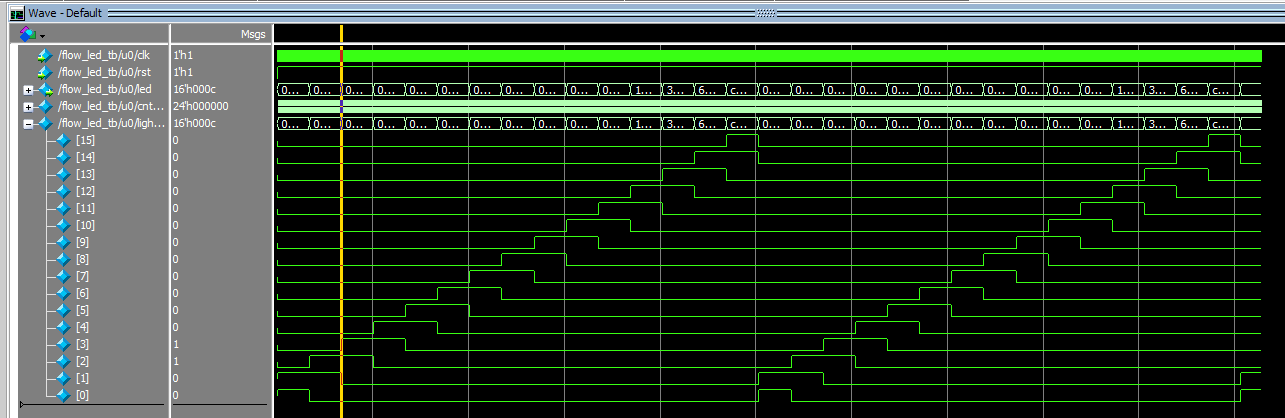
\includegraphics[width=0.7\textwidth]{image/2024-06-28-13-02-04.png}
    \caption{流水灯仿真结果}
    \label{image_led_sim_1}
\end{figure}
流水灯的仿真结果如图\ref{image_led_sim_1}所示, 可以看到16位的LED灯不断流水循环移位。\\
\newpage
\begin{figure}[htbp]
    \centering
    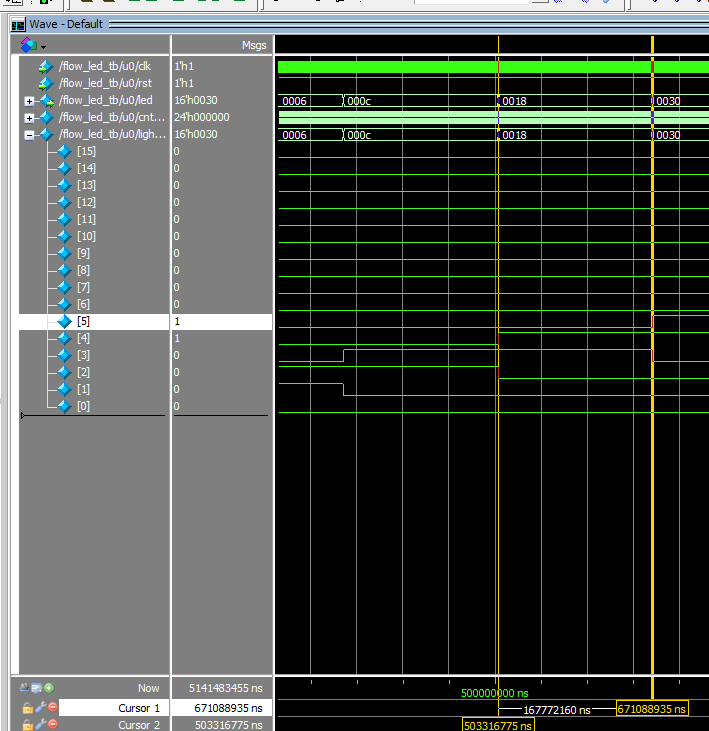
\includegraphics[width=0.7\textwidth]{image/2024-06-28-13-04-00.png}
    \caption{流水灯仿真时序观察}
    \label{image_led_sim_2}
\end{figure}
针对流水灯时序结果的仿真观察如图\ref{image_led_sim_2}所示, 设计的分频器为24位, 对100MHz进行$2^{24}$分频, 分频结果如下所示, 与仿真结果一致。
\begin{equation}
    f = \frac{100*10^6}{2^{24}} \si{\hertz} = \SI{5.96046}{\hertz}
\end{equation}
\begin{equation}
    T = \frac{1}{f} = \SI{0.16777216}{\second}
\end{equation}
% 第四部分
\section*{\fourhao 四、硬件验证结果}
\xiaosihao
\setstretch{1.5}
% 记录加编程器与拨码开关和发光二极管、数码管等的连接情况。记录开发板硬件验证结果,并分析其结果的正确性。
% 按照基础任务、提高任务和拓展任务分别分析
\begin{figure}[htbp]
    \begin{minipage}[t]{0.45\linewidth}
        \centering
        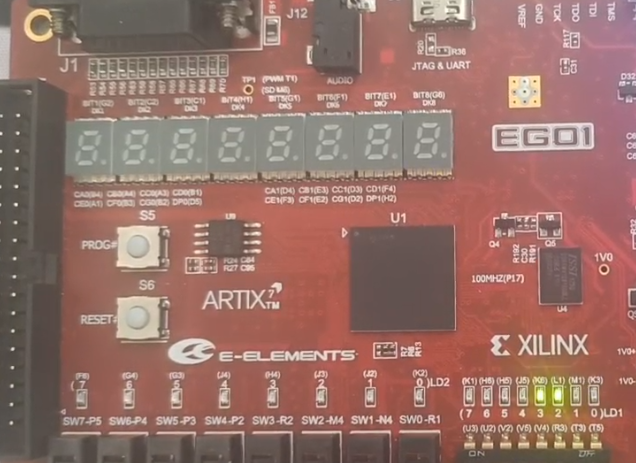
\includegraphics[width=0.7\textwidth]{image/2024-06-28-12-58-06.png}
        \caption{硬件验证}
        \label{image_verify_1}
    \end{minipage}
    \begin{minipage}[t]{0.45\linewidth}
        \centering
        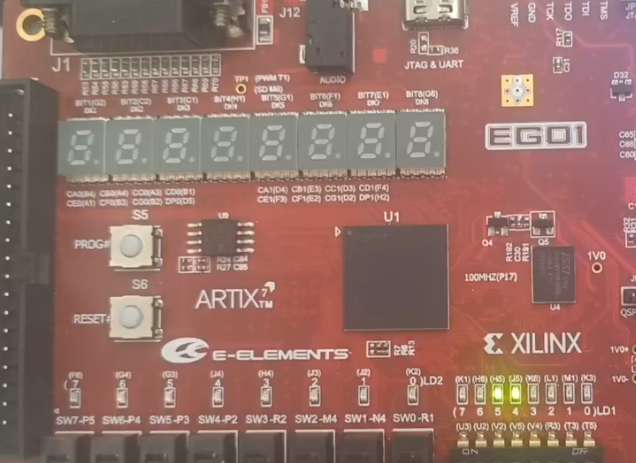
\includegraphics[width=0.7\textwidth]{image/2024-06-28-12-58-21.png}
        \caption{硬件验证}
        \label{image_verify_2}
    \end{minipage}
\end{figure}
硬件验证结果如图图\ref{image_verify_1}和图\ref{image_verify_2}所示,
其中图\ref{image_verify_2}晚于图\ref{image_verify_1}, 可以看到LED两
个点亮, 每次步进一个灯的长度, 循环流水。
% 第五部分
\section*{\fourhao 五、问题解决}
\xiaosihao
\setstretch{1.5}
% 设计过程中遇到的问题及解决的方法。
\subsection*{程序固化到Flash中}
解决: 查阅资料, 多次尝试。Vivado默认的program device是通过jtag口下载程序, 将程序写入FPGA的RAM之中, 重新上电就会丢失。
为了让FPGA重新上电后依然能够运行指定程序, 需要借助FPGA外部的FLASH固化程序, 上电时FPGA从其中读取程序。\\

利用Vivado将程序固化到FLASH需要生成MCS(Memory Configuration File), 在Vivado的tools工具栏中, 
这个文件主要用于指定FLASH类型, 以便PC使用特定的协议与FLASH通信。\\

查阅开发板手册, 手册中写到使用的FLASH为N25Q32 3V3, 进一步查看IC手册, 确定MCS文件生成。\\

烧录失败, 提示检测到的芯片为N25Q64, 检查芯片丝印, 确定为N25Q64,
重新生成MCS固化, 查找原因, N25常用的是SPIx4, 但没办法直接设置, 
因为默认综合产生的bit流文件为SPIx1, 更改SPI位宽设置需要在综合界面的Tcl中执行如下命令完成:
\begin{lstlisting}[language=Verilog]
set_property BITSTREAM.CONFIG.SPI_BUSWIDTH 4 [current_design]
\end{lstlisting}
\begin{figure}[htbp]
    \centering
    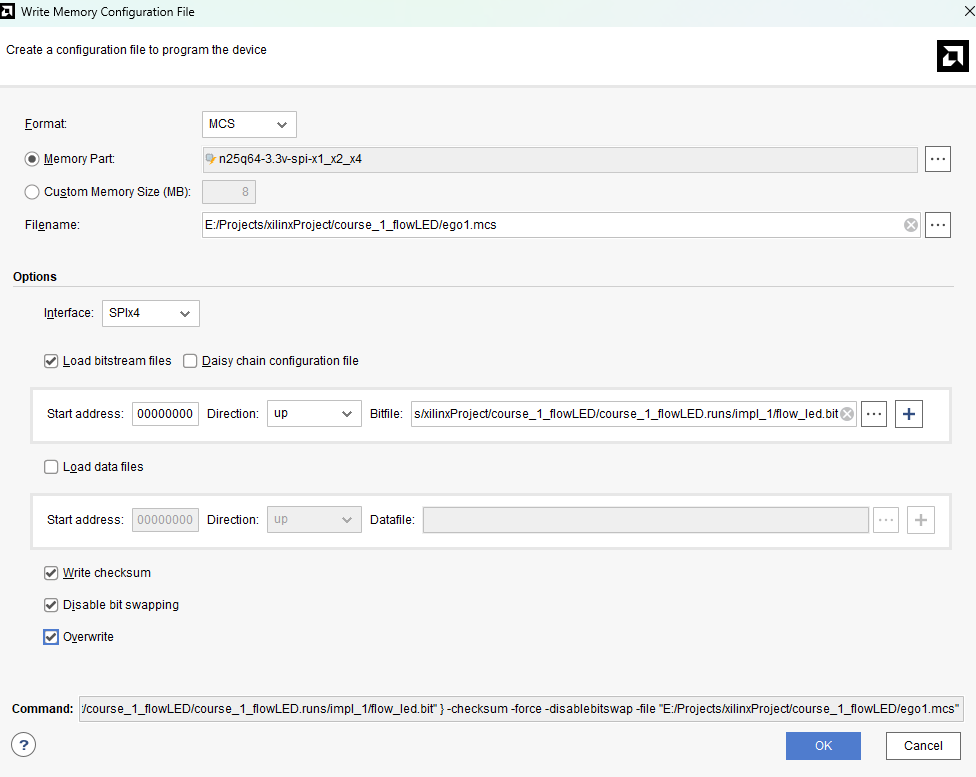
\includegraphics[width=0.7\textwidth]{image/2024-06-30-17-51-50.png}
    \caption{正确的MCS配置}
    \label{image_QA_1}
\end{figure}
重新生成MCS文件如图\ref{image_QA_1}所示, 最终烧录固化成功。
% 第六部分
\section*{\fourhao 六、心得体会}
\xiaosihao
通过一个简单的流水灯设计过程对数字电路基础所学内容进行复习回忆, 掌握Vivado工具的基本使用, 包括使用Vivado综合,
查看综合结果, 查看布局布线结果, 或是进行时序仿真, 通过JTAG接口进行硬件调试, 时序约束和I/O约束等等功能都被集成
到了Vivado工具之中。其中Vivado还提供了IP封装以及Xilinx提供的IP核的配置和调用, 常见的有FIFO, 时钟等IP核的提供。\\

了解到学习通中提供的众多资料中, 有很多是本课程多年积累的成果, 其中很多针对实际问题的案例和解析, 在学习的过程中可以利用
这些资源辅助, 将工程实践的实际问题与理论学习相结合, 可以提高针对工程应用的学习效率。
\end{document}
